\documentclass{beamer}
\usepackage{relsize}
\usepackage{color}

\usepackage{listings}
\usetheme{CambridgeUS}
%\usepackage{beamerthemesplit} % new 
\usepackage{enumitem}
\usepackage{amsmath}                    % See geometry.pdf to learn the layout options. 
\usepackage{amsthm}                   % See geometry.pdf to learn the layout options. There 
\usepackage{amssymb}                    % See geometry.pdf to learn the layout options. 
\usepackage[utf8]{inputenc} 
\usepackage{graphicx}
\usepackage[english,bulgarian]{babel}

\lstset{language=C++,
                basicstyle=\ttfamily,
                keywordstyle=\color{blue}\ttfamily,
                stringstyle=\color{red}\ttfamily,
                commentstyle=\color{green}\ttfamily,
                morecomment=[l][\color{magenta}]{\#}
}

\newtheorem{mydef}{Дефиниция}[section]
\newtheorem{lem}{Лема}[section]
\newtheorem{thm}{Твърдение}[section]

\DeclareMathOperator{\restrict}{\upharpoonright}

\setitemize{label=\usebeamerfont*{itemize item}%
  \usebeamercolor[fg]{itemize item}
  \usebeamertemplate{itemize item}}

\setbeamercovered{transparent}



\begin{document}
\title[Увод в програмирането]{Двумерни масиви и вложени цикли for} 
\author{Калин Георгиев} 
\frame{\titlepage} 


\section{Думерни масиви} 


\begin{frame}
\centerline{Двумерна информация}
\end{frame}



\begin{frame}[fragile]
\frametitle{Таблици}


\begin{center}

\begin{tabular}{ c | c | c }
\hline
  & Мъже & Жени \\\hline
 1990 & 48.75\% & 49.06\% \\\hline
 2000 & 49.06\% & 50.94\% \\\hline
\end{tabular}

\end{center}

\end{frame}


\begin{frame}[fragile]
\frametitle{Матрици}


\begin{equation*}
A=\begin{pmatrix}
  1 & 0 & 0 \\
  0 & 1 & 0 \\
  0 & 0 & 1 
\end{pmatrix}
\end{equation*}

\pause

\begin{equation*}
\begin{pmatrix}
  a_{1,1} & a_{1,2} & a_{1,3} \\
  a_{2,1} & a_{2,2} & a_{3,3} \\
  a_{3,1} & a_{3,2} & a_{3,3} 
\end{pmatrix}
\end{equation*}


\end{frame}


\begin{frame}[fragile]
\frametitle{Двумерни масиви}

\begin{lstlisting}
int a[3][3];
\end{lstlisting}

\pause

\begin{center}

  
\begin{tabular}{ | c | c | c |}
\hline
a[0][0] & a[0][1] & a[0][2] \\\hline
a[1][0] & a[1][1] & a[1][2] \\\hline
a[2][0] & a[2][1] & a[2][2] \\\hline
  
\end{tabular}

\pause

\begin{equation*}
\begin{pmatrix}
  a_{1,1} & a_{1,2} & a_{1,3} \\
  a_{2,1} & a_{2,2} & a_{3,3} \\
  a_{3,1} & a_{3,2} & a_{3,3} 
\end{pmatrix}
\end{equation*}



\end{center}




\end{frame}


\begin{frame}[fragile]
\frametitle{Двумерни масиви в паметта}


\begin{lstlisting}
int a[3][3];
\end{lstlisting}

\pause

\begin{flushleft}

\relscale{0.6}

\begin{tabular}{ | c | c | c |}
\hline
a[0][0] & a[0][1] & a[0][2] \\\hline
a[1][0] & a[1][1] & a[1][2] \\\hline
a[2][0] & a[2][1] & a[2][2] \\\hline
  
\end{tabular}
\end{flushleft}

\pause

\begin{center}
\relscale{0.7}
\begin{tabular}{  c | c | c | c | c | c | c | c | c | c | c }
\hline
...&0&1&2&3&4&5&6&7&8&... \\\hline
...&
a[0][0] & a[0][1] & a[0][2] &
a[1][0] & a[1][1] & a[1][2] &
a[2][0] & a[2][1] & a[2][2] &
... \\\hline
  
\end{tabular}


\end{center}

\pause

\begin{itemize}
\item $index = row * 3 + column$
\end{itemize}



\end{frame}


\begin{frame}[fragile]
\frametitle{Операции с двумерни масиви}

\begin{itemize}
  \item Дефиниране чрез тип и измерения: 

\begin{lstlisting}
int arr[10][50];
\end{lstlisting}
\pause
  \item Достъп до всеки отделен елемент:

\begin{lstlisting}
int b = arr[1][2];
cin >> arr[3][5];
b = arr[4][1] + arr[2][1];
\end{lstlisting}


\end{itemize}

\end{frame}



\begin{frame}[fragile]
\frametitle{Обхождане на фиксиран ред}

\begin{flushleft}
\relscale{0.7}

\begin{lstlisting}
for (int colCount = 0; colCount < 4; colCount++)
{
  cout << "arr[2][" 
       << rowCount << "]=";
  
  cin >> arr[2][colCount];
}
\end{lstlisting}
\end{flushleft}

\vspace*{-120pt}
%\hspace*{-30pt}
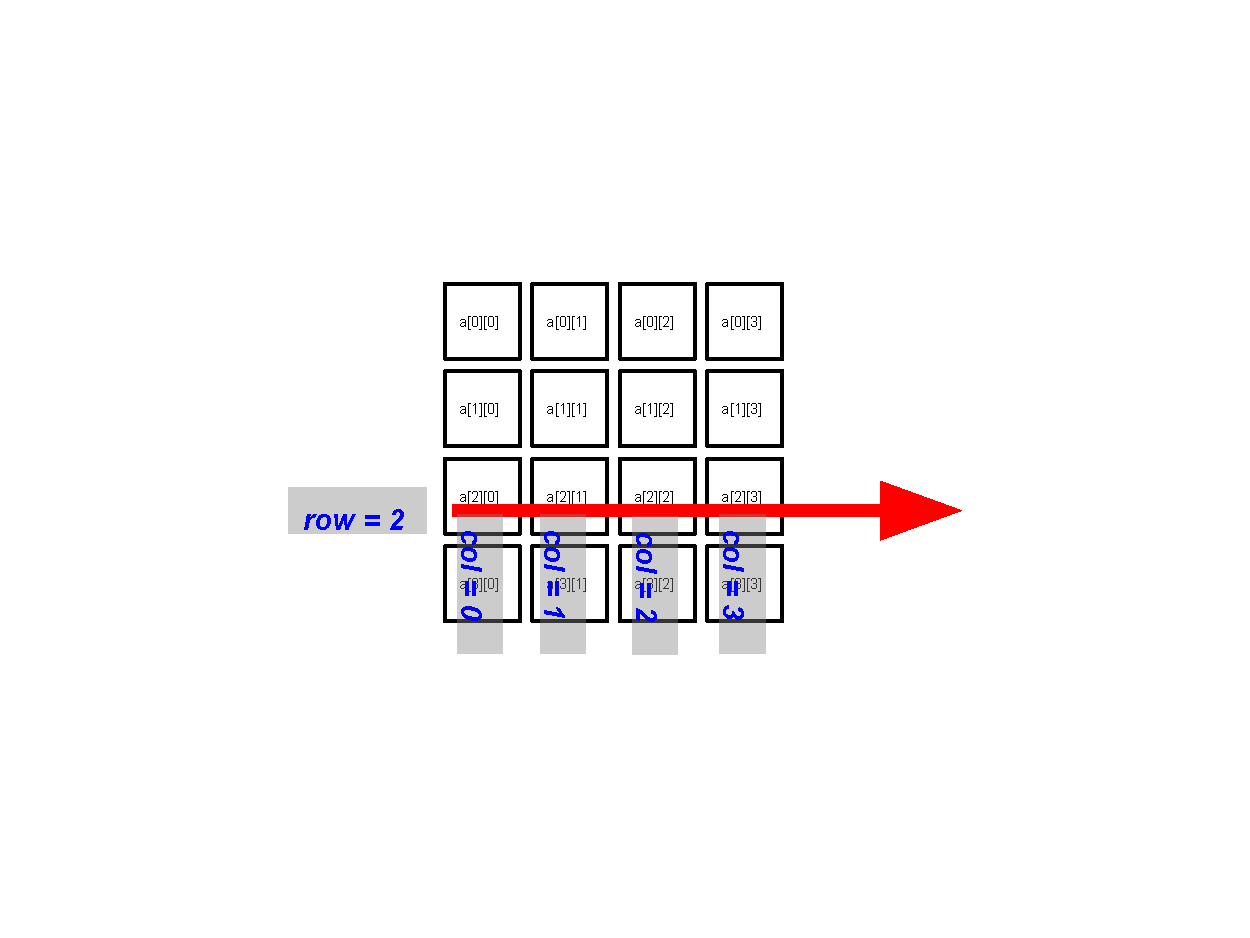
\includegraphics[width=14cm]{images/matr_iter_cols} 

\end{frame}

\begin{frame}[fragile]
\frametitle{Обхождане на всички редове}

\begin{flushleft}
\relscale{0.7}

\begin{lstlisting}
for (int rowCount = 0, rowCount < 4; rowCount++)
{
  .........
}
\end{lstlisting}
\end{flushleft}

\vspace*{-100pt}
%\hspace*{-30pt}
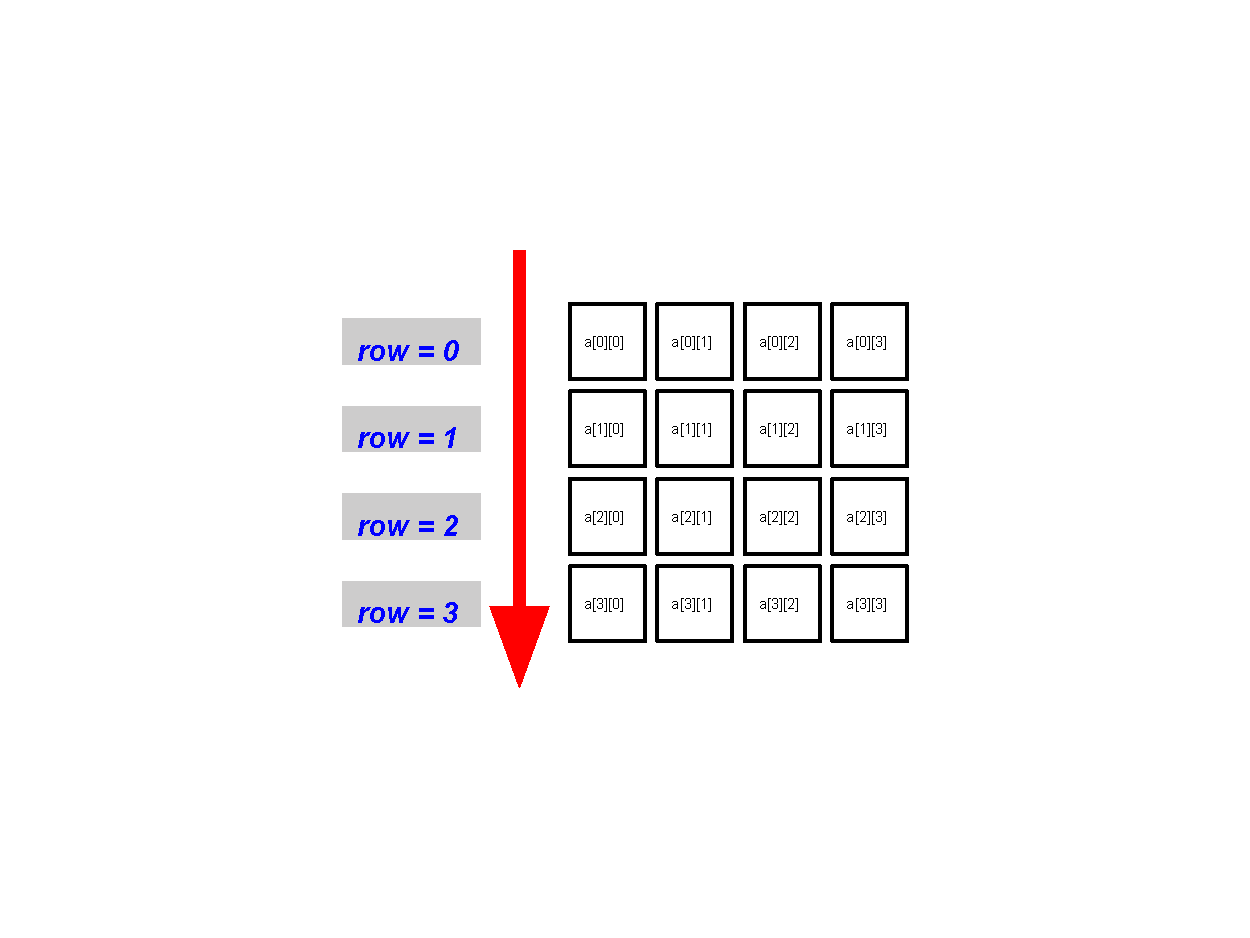
\includegraphics[width=14cm]{images/matr_iter_rows} 

\end{frame}


\begin{frame}[fragile]
\frametitle{Обхождане}

\begin{flushleft}
\relscale{0.67}

\begin{lstlisting}
for (int rowCount = 0, rowCount < 4; rowCount++)
{
  for (int colCount = 0; colCount < 4; colCount++)
  {
    cout << "arr["
         << rowCount << "]["
         << colCount << "]="; 
    
    cin >> arr[rowCount][colCount];
  }
}
\end{lstlisting}
\end{flushleft}

\vspace*{-100pt}
\hspace*{-40pt}
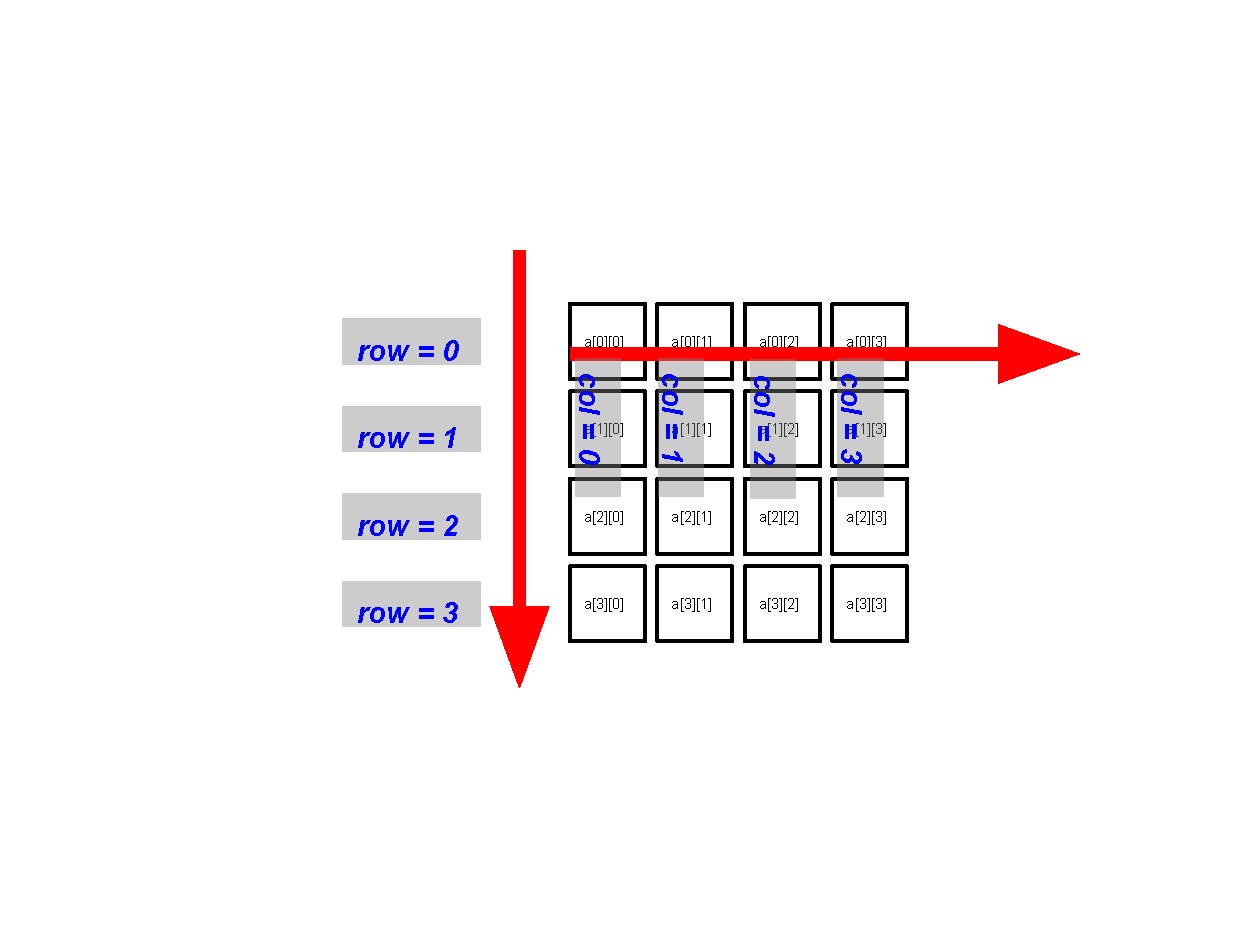
\includegraphics[width=12cm]{images/matr_iter_0} 

\end{frame}

\begin{frame}[fragile]
\frametitle{Обхождане}

\begin{flushleft}
\relscale{0.67}

\begin{lstlisting}
for (int rowCount = 0, rowCount < 4; rowCount++)
{
  for (int colCount = 0; colCount < 4; colCount++)
  {
    cout << "arr["
         << rowCount << "]["
         << colCount << "]="; 
    
    cin >> arr[rowCount][colCount];
  }
}
\end{lstlisting}
\end{flushleft}

\vspace*{-100pt}
\hspace*{-40pt}
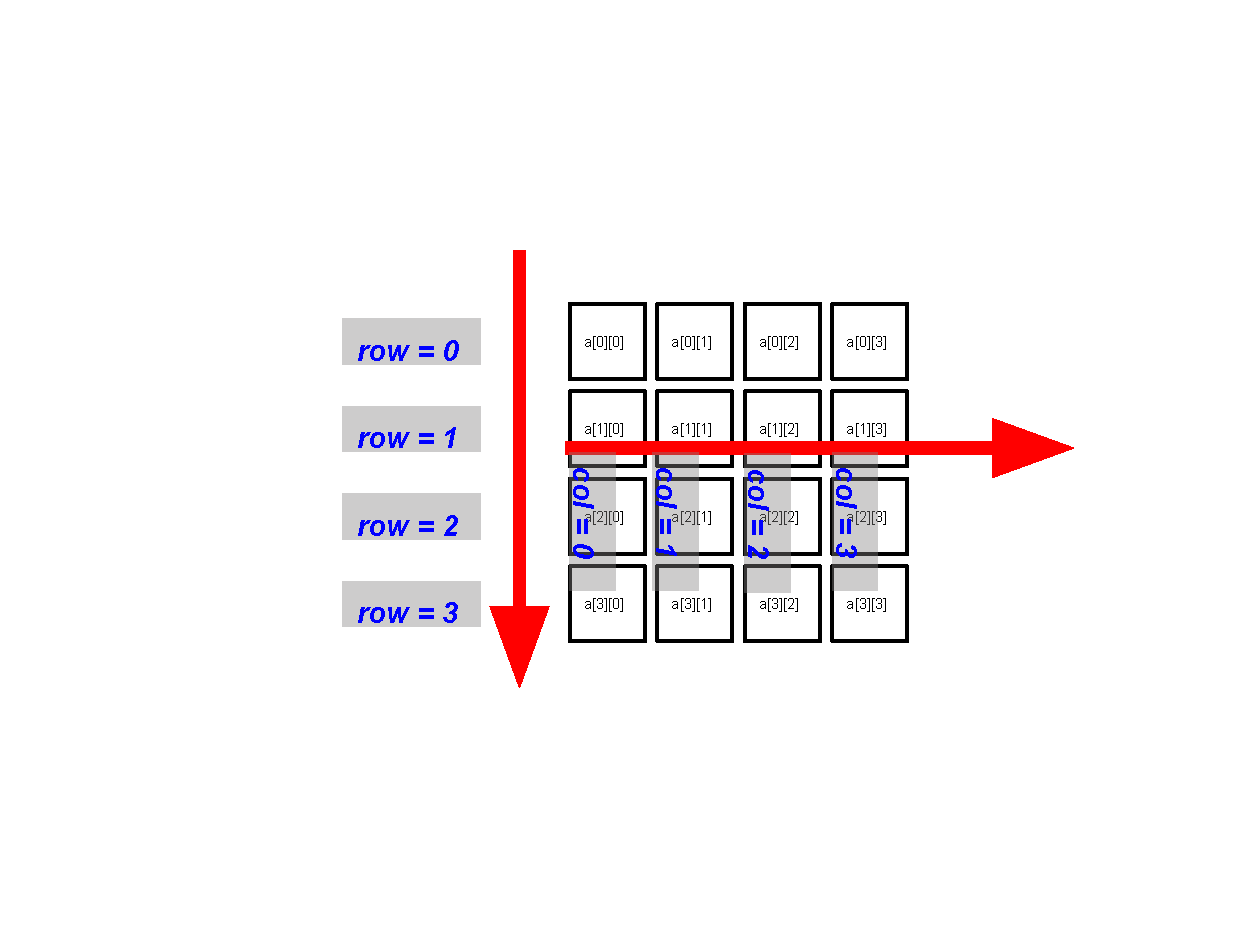
\includegraphics[width=12cm]{images/matr_iter_1} 

\end{frame}

\begin{frame}[fragile]
\frametitle{Обхождане}

\begin{flushleft}
\relscale{0.67}

\begin{lstlisting}
for (int rowCount = 0, rowCount < 4; rowCount++)
{
  for (int colCount = 0; colCount < 4; colCount++)
  {
    cout << "arr["
         << rowCount << "]["
         << colCount << "]="; 
    
    cin >> arr[rowCount][colCount];
  }
}
\end{lstlisting}
\end{flushleft}

\vspace*{-100pt}
\hspace*{-40pt}
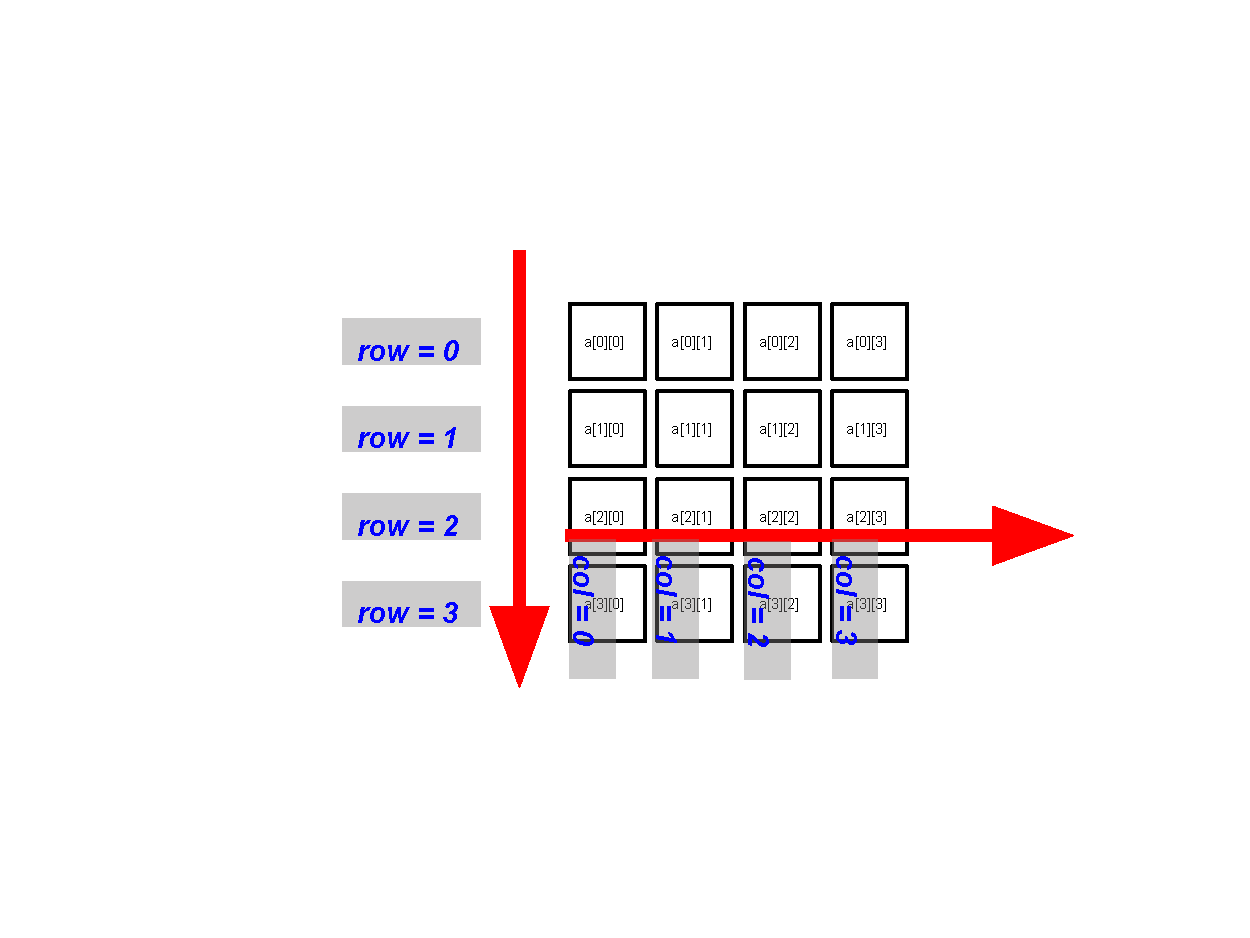
\includegraphics[width=12cm]{images/matr_iter_2} 

\end{frame}

\begin{frame}[fragile]
\frametitle{Обхождане}

\begin{flushleft}
\relscale{0.67}

\begin{lstlisting}
for (int rowCount = 0, rowCount < 4; rowCount++)
{
  for (int colCount = 0; colCount < 4; colCount++)
  {
    cout << "arr["
         << rowCount << "]["
         << colCount << "]="; 
    
    cin >> arr[rowCount][colCount];
  }
}
\end{lstlisting}
\end{flushleft}

\vspace*{-100pt}
\hspace*{-40pt}
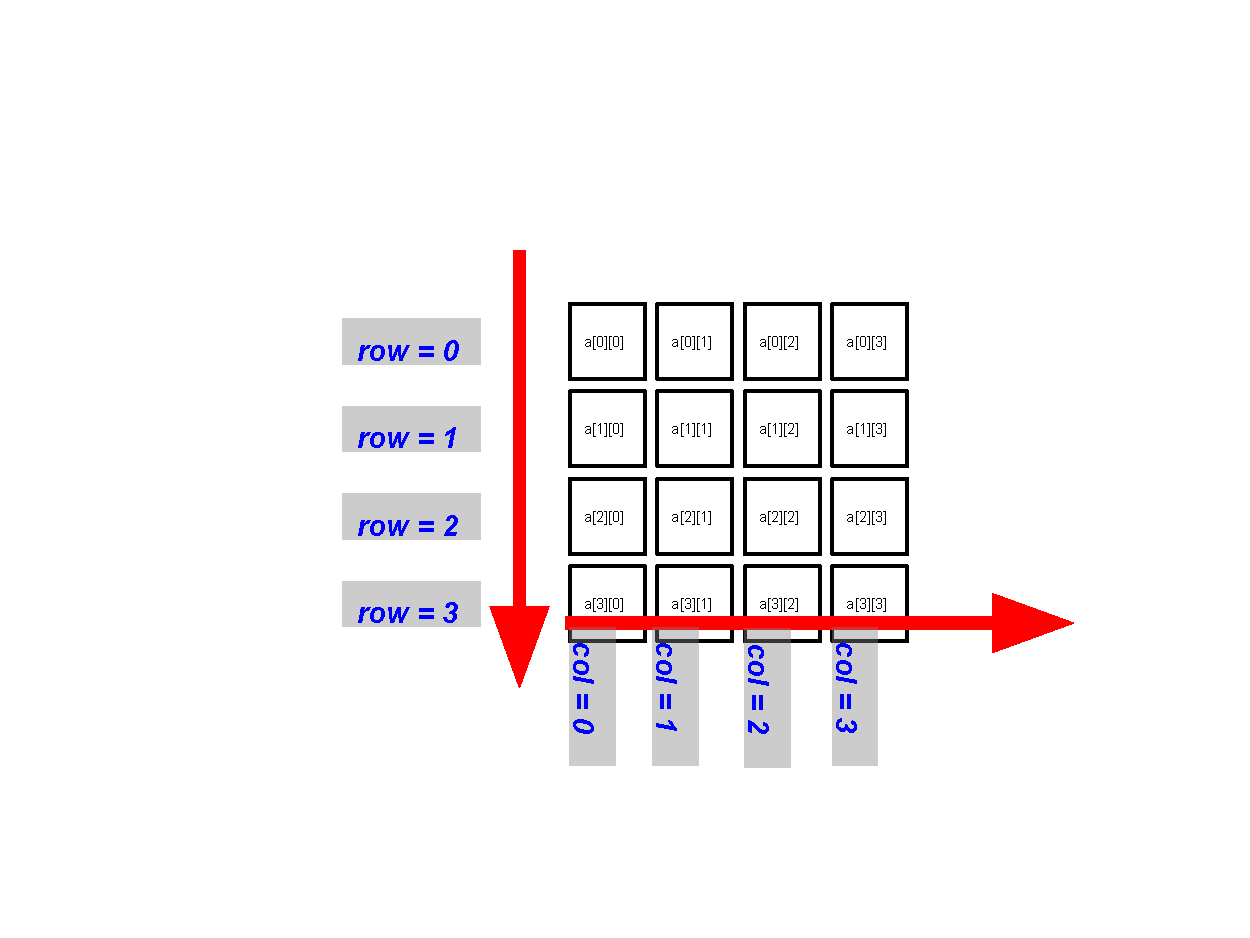
\includegraphics[width=12cm]{images/matr_iter_3} 

\end{frame}

\begin{frame}
\centerline{Благодаря за вниманието! }
\end{frame}

\end{document}


\begin{columns}[t]
  \begin{column}{0.2\textwidth}

  \end{column}
  \begin{column}{0.8\textwidth}

  \end{column}
\end{columns}


